\documentclass{article}
<<<<<<< HEAD
\usepackage{ugentstyle}

\usepackage{graphicx}
\usepackage{subcaption}
\graphicspath{{img/}}

=======
\usepackage{listings}
\usepackage{hyperref}
\usepackage{subcaption}
\usepackage{graphicx}
\usepackage[a4paper, total={6in, 9in}]{geometry}
\graphicspath{{./}}
>>>>>>> 818f09473b0ac2110ec294254a476bf5dbf0865f


\begin{document}
	\title{Lab 4: Bounds Check Analysis}
	\author{Bert De Saffel, Xandro Vermeulen}
	\maketitle
	\tableofcontents
	
	\section{Introduction}
	This report describes the performance of three different \texttt{IR} representations of a single \texttt{C} program, \texttt{bubble\_sort.c}. The first \texttt{IR} representation is the standard representation without a function pass. The second implementation modifies the \texttt{IR} by applying bound checking using branch instructions for each \texttt{getelementptr} instruction. The third representation also applies bound checking, but with an extra optimalisation: 
	
	\section{Modification of the IR}
<<<<<<< HEAD
	Before the analysis is explained, a description of the transformations made to the IR are described. To demonstrate, a simple $C$ program is used:
	\begin{lstlisting}
=======
	When implementing runtime bounds checking, transformations to the IR have to be made as the default IR does not handle runtime bounds checking. To demonstrate the changes, a simple $C$ program is used:
	\begin{lstlisting}[numbers=left]
>>>>>>> 818f09473b0ac2110ec294254a476bf5dbf0865f
int foo[10];
int n = 9;
foo[n] = 5;
foo[n + 1] = 5;
	\end{lstlisting}
<<<<<<< HEAD
The second array indexing must result in a runtime error. The original IR is shown next to the modified IR in figure 
\begin{figure}[h!]
	\centering
	\begin{subfigure}[b]{0.4\linewidth}
		\includegraphics[width=\linewidth]{fig_overflow.jpg}
		\caption{Coffee.}
	\end{subfigure}
	\begin{subfigure}[b]{0.4\linewidth}
		\includegraphics[width=\linewidth]{fig_overflow.jpg}
		\caption{More coffee.}
	\end{subfigure}
	\caption{The same cup of coffee. Two times.}
	\label{fig:coffee}
\end{figure}

=======
The second array indexing on line 4 should result in a runtime error. The original and modified IR are shown respectively on figure \ref{fig:original_ir} and \ref{fig:modified_ir}. The IR on figure \ref{fig:original_ir} will simply give a segmentation fault when line 4 is executed. To combat this, each \texttt{getelementptr} instruction is preceded by a \texttt{icmp} instruction, which compares the index value with the array size, and a \texttt{br} instruction which will chose the \texttt{trap} or \texttt{cont} block based on the resulting boolean value of the \texttt{icmp} instruction. The resulting IR is shown on figure \ref{fig:modified_ir}.

\begin{figure}
	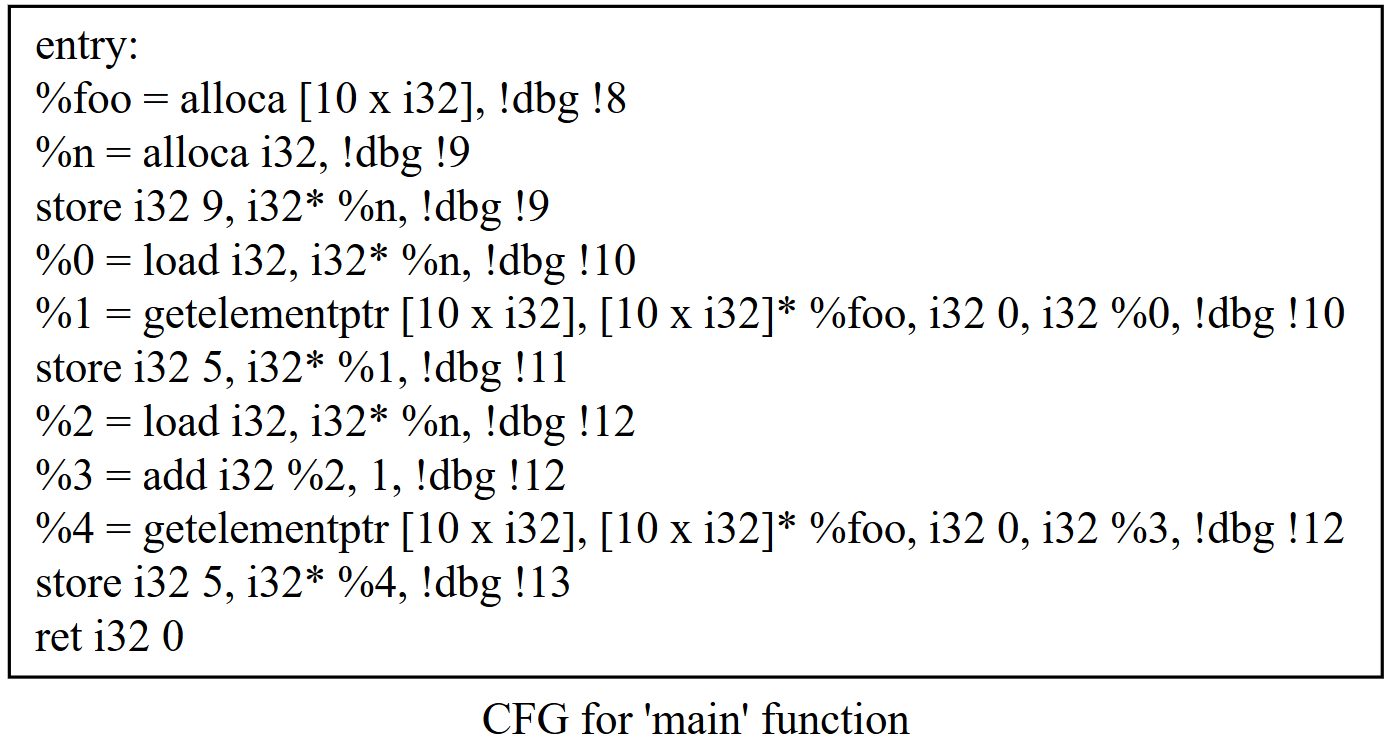
\includegraphics[width=\linewidth]{fig_overflow}
	\caption{The original, unmodified IR for program REF.}
	\label{fig:original_ir}
\end{figure}

\begin{figure}
	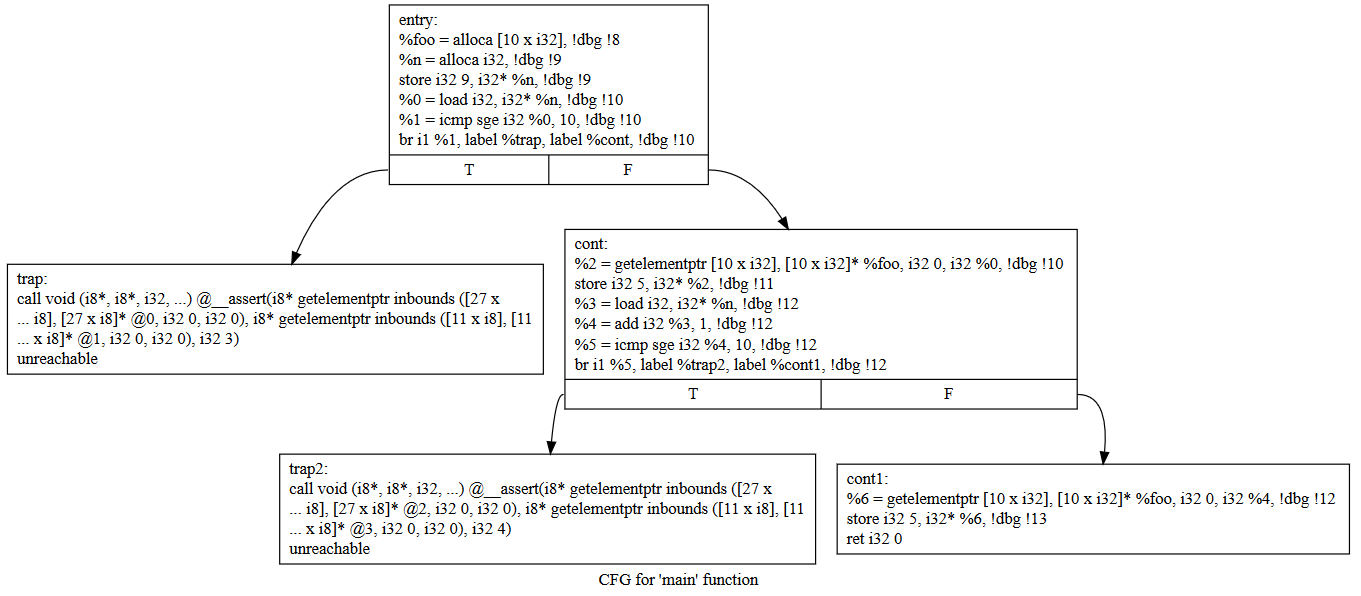
\includegraphics[width=\linewidth]{fig_overflow_checked}
	\caption{Modified IR for program REF.}
	\label{fig:modified_ir}
\end{figure}



>>>>>>> 818f09473b0ac2110ec294254a476bf5dbf0865f
	\section{Analysis}
	Using the method above, a program that contains $n$ \texttt{getelementptr} instructions will contain $2n$ extra basic blocks, $n$ extra \texttt{icmp} instructions and $n$ extra \texttt{br} instructions. To measure the impact of these extra instructions and basic blocks, the program \texttt{bubble\_sort.c} is executed 30 times for both representations. Afterwards, average statistics such as runtime can be calculated for each representation. It can be assumed that inserting more code to perform the runtime bounds checking will increase performance overhead. Indeed, the average runtime for the original and modified representation is respectively \texttt{2758 ms} and \texttt{3141 ms}, resulting in a 13\% increase for the modified version. This has a straightforward explanation: each \texttt{getelementptr} is preceded by a \texttt{icmp} and \texttt{br} instruction. To explain this, we consider line 33 of \texttt{bubble\_sort.c}, which contains the following code:
	$$\texttt{a = numbers[j]}$$
 	The generated assembly code is shown on figure \ref{fig:machine_code}. This shows how the value of $j$, which resides at an offset of $4$ bytes from the base pointer, is put in the \texttt{\%RAX} register. Then the array \texttt{numbers} is accessed by calculating the correct address and putting the value which resides at this address in the \texttt{\%ECX} register. This value is then put into the variable $a$, which resides at an offset of 28 ($0x1c$) bytes from the base pointer. Now compare this to figure \ref{fig_machine_code_checked}, which contains 3 new instructions as a result of the runtime bounds check. The first instruction is a \texttt{cmp} instruction, which compares the maximum array offset (0x1ff = 511)  to the index value (the $j$ variable). The second instruction is a \texttt{jg} instruction, which jumps to its corresponding \texttt{trap} block if the previous \texttt{cmp} instruction holds true ($j > 511$). A third instruction is \texttt{cltq}, which converts the value in the \texttt{EAX} register from a long (4 bytes) to a quad (8 bytes). This conversion is neccesary because the register \texttt{\%EAX} is a 32-bit register and the following operations use 64-bit registers. The word length of each register in an instruction must be equal. Of these three new instructions, the \texttt{cltq} instruction takes the most time.
 	
 	 However, this could be avoided if a 64-bit integer type was used in the IR instead of a 32-bit integer type. Unfortunately, this requires that the source program also uses unsigned integers.
	
	\begin{figure}
		\centering
		\begin{subfigure}{0.48\textwidth}
			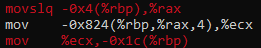
\includegraphics[width=\linewidth]{fig_machine_code}
			\caption{Generated assembly code for the original IR.}
			\label{fig:machine_code}
		\end{subfigure}
		\begin{subfigure}{0.48\textwidth}
			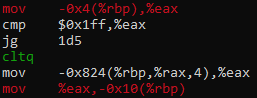
\includegraphics[width=\linewidth]{fig_machine_code_checked}
			\caption{Generated assembly code for the modified IR.}
			\label{fig_machine_code_checked}
		\end{subfigure}
		\caption{x86-64 assembly code for line 33 in \texttt{bubble\_sort.c}.}
	\end{figure}
	
	
	\subsection{Optimalisation}
\end{document}